% Exemplo de relatório técnico do IC
% Criado por P.J.de Rezende antes do Alvorecer da História.
% Modificado em 97-06-15 e 01-02-26 por J.Stolfi.
% Last edited on 2003-06-07 21:12:18 by stolfi

% modificado em 1o. de outubro de 2008

\documentclass[11pt,twoside]{article}
\usepackage{techrep-ic}
\usepackage[pdftex]{graphicx}
\usepackage{enumerate}

%%% SE USAR INGLÊS, TROQUE AS ATIVAÇÕES DOS DOIS COMANDOS A SEGUIR:
\usepackage[brazil]{babel}
%% \usepackage[english]{babel}

%%% SE USAR CODIFICAÇÃO LATIN1, TROQUE AS ATIVAÇÕES DOS DOIS COMANDOS A
%%% SEGUIR:
%% \usepackage[latin1]{inputenc}
\usepackage[utf8]{inputenc}

\begin{document}

%%% PÁGINA DE CAPA %%%%%%%%%%%%%%%%%%%%%%%%%%%%%%%%%%%%%%%%%%%%%%%
%
% Número do relatório
\TRNumber{45}

% DATA DE PUBLICAÇÃO (PARA A CAPA)
%
\TRYear{10} % Dois dígitos apenas
\TRMonth{06} % Numérico, 01-12

% LISTA DE AUTORES PARA CAPA (sem afiliações).
\TRAuthor{Birocchi, Anderson - RA: 072787 \and Braga, Felipe - RA:070803}

% TÍTULO PARA A CAPA (use \\ para forçar quebras de linha).
\TRTitle{MC823 - Laboratório de Redes\\Projeto 3: Sistema RMI para Consulta a Dados de um Cinema}

\TRMakeCover

%%%%%%%%%%%%%%%%%%%%%%%%%%%%%%%%%%%%%%%%%%%%%%%%%%%%%%%%%%%%%%%%%%%%%%
% O que segue é apenas uma sugestão - sinta-se à vontade para
% usar seu formato predileto, desde que as margens tenham pelo
% menos 25mm nos quatro lados, e o tamanho do fonte seja pelo menos
% 11pt. Certifique-se também de que o título e lista de autores
% estão reproduzidos na íntegra na página 1, a primeira depois da
% página de capa.
%%%%%%%%%%%%%%%%%%%%%%%%%%%%%%%%%%%%%%%%%%%%%%%%%%%%%%%%%%%%%%%%%%%%%%

%%%%%%%%%%%%%%%%%%%%%%%%%%%%%%%%%%%%%%%%%%%%%%%%%%%%%%%%%%%%%%%%%%%%%%
% Nomes de autores ABREVIADOS e titulo ABREVIADO,
% para cabeçalhos em cada página.
%
\markboth{Birocchi, Braga}{MC823 - Projeto 3, Aplicação RMI}
\pagestyle{myheadings}

%%%%%%%%%%%%%%%%%%%%%%%%%%%%%%%%%%%%%%%%%%%%%%%%%%%%%%%%%%%%%%%%%%%%%%
% TÍTULO e NOMES DOS AUTORES, completos, para a página 1.
% Use "\\" para quebrar linhas, "\and" para separar autores.
%
\title{MC823 - Projeto 3, Sistema RMI para Consulta a Dados de um Cinema}

\author{Anderson Birocchi, Felipe Braga}

\date{}

\newpage
\tableofcontents
\newpage

\maketitle

%%%%%%%%%%%%%%%%%%%%%%%%%%%%%%%%%%%%%%%%%%%%%%%%%%%%%%%%%%%%%%%%%%%%%%

\newenvironment{codelisting}
{\begin{list}{}{
\setlength{\leftmargin}{1em}
}
\item\scriptsize\bfseries}{\end{list}}


\begin{abstract}
Este projeto consiste da implementação de um sistema de comunicação em rede, baseado no paradigma cliente-servidor, motivado pela provisão de acesso a uma base de dados de filmes. Para a comunicação entre cliente e servidor, foi utilizado o Java RMI - \textit{Remote Method Invocation}. Foram ainda realizadas análises quanto ao desempenho da aplicação e uma comparação desse sistema de mais alto nível com o sistema do projeto anterior, implementado em C, a um nível de abstração mais baixo.
\end{abstract}

\section{Introdução}
Nos dia de hoje é comum se ter qualquer tipo de informação de forma rápida e prática através da internet, como mapas, receitas, notícias, preços de mercado, cotação das moedas do mundo todo, etc. De tudo que se pode fazer pela internet, a área que mais cresce é a de prestação de serviços, onde já se pode fazer compras, pagar contas, fazer transações bancárias dentre várias outras coisas, e um desses tipos de serviço será implementado pelo nosso projeto.\\
Nosso projeto irá implementar um servidor Java multi-usuário utilizando RMI para comunicação e SQL para consultas em banco de dados de um cinema, onde são armazenadas várias informações sobre os filmes em cartaz, como o título, sinopse, horário das sessões e as salas.\\
O intuito é de centralizar as informações dos filmes em um único local, evitando que cada cliente tenha que ficar se sincronizando toda vez que for fazer uma consulta; além de tornar o programa cliente leve e livre da carga de processamento necessário para as consultas, permitindo assim que aparelhos com poder de processamento menor como celulares ou palm-tops também possam executar o programa sem problemas.\\
Iremos criar os 2 aplicativos, o servidor e o cliente, e também criaremos o protocolo de comunicação entre os 2, e esse protocolo será baseado em objetos invocados remotamente através do Java RMI.\\
A seção 2 irá especificar o que exatamente o programa deve fazer; a seção 3 irá comentar mais detalhadamente a implementação, as definições, suposições tomadas e ferramentas utilizadas; a seção 4 irá analisar o desempenho da aplicação atraveś de várias medidas de tempo; a seção 5 irá mostrar quão confiável e consistente é a aplicação; na seção 6 encontra-se uma breve conclusão sobre o projeto e, por último, na seção 7 estará o código fonte necessário para compilar e executar o servidor e o cliente.


\section{Casos de Uso}
Primeiramente, devemos especificar o que a aplicação deve fazer, portanto segue abaixo uma listagem de 6 ações que serão implementadas. Nota: as ações com (*) precisam receber um identificador numérico do filme como entrada.\\
As ações sempre serão tomadas pelo cliente, sendo o servidor apenas quem irá processar o pedido. O resultado da ação apenas é vista pelo cliente que a iniciou, deixando o servidor totalmente à parte do que está acontecendo do lado dos seus clientes.
\subsection{Listar todas as informações de todos os filmes}
Mostrar o ID, título, sinopse, horário das sessões e as salas de todos os filmes cadastrados no banco de dados do servidor.
\subsection{Listar ID e título de todos os filmes}
Fazer uma busca rápida de todos os títulos e seus IDs, mais utilizado para auxiliar em futuras consultas, e utilização dos próximos casos de uso.
\subsection{Listar todas as informações de um filme (*)}
Buscar todas as informações sobre o filme com o dado ID.
\subsection{Mostrar a sinopse de um filme (*)}
Mostrar a sinopse completa do filme com o dado ID.
\subsection{Mostrar a avaliação de um filme (*)}
Mostrar a quantidade de votos o filme teve e qual foi a pontuação obtida.
\subsection{Avaliar um filme (*)}
Dar uma pontuação ao filme com o dado ID.


\section{Implementação}
O sistema é desenvolvido na linguagem Java, utiliza as bibliotecas RMI "java.rmi.*" para fazer a comunicação pela rede e gerencia as várias conexões automaticamente, conseguido pelo alto nível de abstração oferecida pela linguagem Java.\\
Primeiramente vamos explicar como foi implementado o banco de dados e suas operações, e depois explicar como é feita a comunicação entre o servidor e o cliente e como é feita a comunicação entre eles.\\
Basicamente, o funcionamento do sistema é: o servidor é um objeto instanciado na máquina virtual Java que publica seus métodos para serem acessados remotamente e aguarda requisições de conexão; o cliente procura pelo servidor através dp RMI Registry no endereço especificado, que libera o acesso do cliente ao servidor; inicia-se uma sequencia de requisições do cliente e respostas por parte do servidor; cliente encerra o uso.\\

%Ao terminar o projeto, fazer um word count e ver quantas linhas deu, e fazer um comentário
No fim, a quantidade de linhas de código de todos os arquivos do sistema (*.java) é 561, o que já não é um programa simples, porém ainda está longe de ser uma grande aplicação.\\

Para organizar a discussão sobre a implementação, vamos tratar de tópicos separamente.\\

\subsection{Banco de Dados}
Utilizamos o SQLite, uma plataforma que implementa as funcionalidades básicas de um SGDB relacional, mas de modo mais simples. Ela utiliza um único arquivo para o banco (que chamamos de filmes.db). A definição dos dados é apresentada na seção do código do sistema, no arquivo tabelas.sql.\\
O uso deste software nos deu duas facilidades: a facilidade de comunicação com a camada de persistência (uso de SQL para consultas e alterações nos dados) e a transparência quanto à garantia de acesso concorrente aos dados.\\
Destaca-se, para este último ponto, o uso do \textit{Driver} para conexão com o banco de dados: sqlitejdbc.jar. Cada conexão aberta pelo servidor é como um programa sqlite3 rodando a partir do arquivo do banco de dados. Assim, a exclusão mútua para as operações de escrita no banco é garantida tanto pela descrição da conexão do JDBC como pelo tratamento de conexões por parte do SQLite.\\
Com relação à implementação, foi criado um pacote chamado bd, com as classes:
\begin{itemize}
  \item ConnectionFactory: implementa a abstração para estabelecimento de conexão com o banco de dados.
  \item DataAccess: abstração para o acesso aos dados do banco. É onde são utilizados os comandos SQL.
  \item Filme: mapeia o tipo de dado da tabela filme para o sistema.
\end{itemize}


\subsection{Comunicação Cliente-Servidor}
Utilizando-se da Orientação a Objetos, propriedade intrínsica da linguagem Java, pudemos implementar a aplicação a partir de um nível muito mais alto de abstração. A saber, temos duas classes principais: Cliente e Servidor. A abstração está no fato de que o objeto cliente utiliza o objeto remoto servidor como se fosse um objeto local. Dessa forma, a partir do momento que o cliente estabelece conexão com o objeto remoto do servidor (a partir do \textit{Registry}), as chamadas aos métodos remotos são transparentes ao cliente. Uma rápida observação é que, numa aplicação grande, que realmente pode acontecer de um programador não saber que se trata de um objeto remoto, pode-se fazer invocações de métodos de forma muito custosa.\\
A classe Servidor implementa a interface RequestInterface, que por sua vez extende Remote. Desse modo, os métodos assinados em RequestInterface, e que são implementados no Servidor, são os métodos que ficam disponíveis a serem executados remotamente. Isso se dá com o cliente também tendo acesso a RequestInterface, mas ao instanciar de fato o objeto que implementa a interface, é feito o acesso à estrutura do RMI.\\
Com a conexão estabelecida, o cliente simplesmente solicita requisições ao objeto servidor em forma de chamadas de método. Os parâmetros são os dados de entrada que o servidor precisa saber para a tarefa que o cliente quer; e o retorno corresponde às informações que o servidor dá ao cliente. Para facilitar a transparência na classe Cliente, foi criada uma classe que define métodos auxiliares: ClientAux.\\
O servidor também utiliza de uma classe auxiliar, DataAccess, que implementa a forma como os dados são acessados no banco. O pacote bd contem as classes ConnectionFactory, DataAccess e Filme. Todas são utilizadas pelo servidor, e apenas Filme é usada pelo cliente, para a definição dos atributos que correspondem a um filme e funções para impressão dos dados.\\
Existem duas requisições que solicitam filmes: todos os filmes do banco ou apenas um a partir de um ID. Nos dois casos, por facilidade de implementação, é retornada uma lista de filmes. Já que o ID entrado no cliente pode não corresponder a nenhum filme, a lista pode voltar vazia. Por fim, existe ainda o método remoto correspondente à avaliação, que recebe o ID e a nota do cliente, e retorna um Booleano, para o caso do filme não existir (retorno False).\\
Como comentado anteriormente, com a transparência da exclusão mútua para os acessos de escrita, a implementação ficou bem concisa e robusta, de modo que até pelo número de linhas de código ficou clara a simplicidade gerada também pela abstração do RMI.\\
Uma última observação, utilizamos um arquivo de definição das políticas de segurança \textit{policy}, apenas como exemplo de uso (já que o fizemos para permitir todos os acessos). A forma como a aplicação é executada pode ser vista nos scripts runserver.sh e runclient.sh.


\section{Análise de Tempo}
Para a análise de tempo, foram consideradas duas operações a serem analisadas: tempo de comunicação (RTT) e requisição ao servidor.\\
Uma coisa importante a se notar é que para calcular o tempo real de requisição ao servidor, temos que subtrair o tempo gasto pelo servidor para realizar a consulta ao bando de dados SQL.\\
Para se obter uma boa precisão, foi utilizada a função "System.nanoTime()", que tem a precisão em nanosegundos, que será convertida em microsegundos, o que é boa o suficiente para nossa aplicação. A função pega o tempo atual em que foi chamada, portanto, para calcular o tempo de alguma operação, basta calcular o tempo antes e depois da operação e calcular a diferença entre eles.\\
Foram feitas 5 análises, cada uma feita em um computador diferente, em salas diferentes, e todos logados com o computador principal da rede do IC3\\
IP local 1: 143.106.16.35 (sala 303)\\
IP local 2: 143.106.16.198 (sala 304)\\
IP local 3: 143.106.16.3 (sala 302)\\
IP local 4: 143.106.16.104(sala 317)\\
IP local 5: 143.106.16.81 (sala 305)\\
IP remoto: 143.106.16.163 (xaveco)\\

\textit{Observação: }Todos os tempos que serão mostrados nas próximas seções estão em micro-segundos, e pode-se verificar todos os valores encontrados nas tabelas da seção de Anexos. Os scripts de teste estão na seção do código fonte.\\

\subsection{Tempo de Comunicação}
Tempo decorrido para realizar a conexão (RTT) e tempo total decorrido para o servidor responder a requisição do cliente.\\

\textbf{Análise 1: }\\
Média do tempo de RTT: \textbf{1346 us}\\
Desvio padrão RTT: \textbf{178 us}\\
Média do tempo total de requisição: \textbf{2011 us}\\
Desvio padrão de requisição: \textbf{572 us}\\
\begin{figure}[htb]
  \centering
  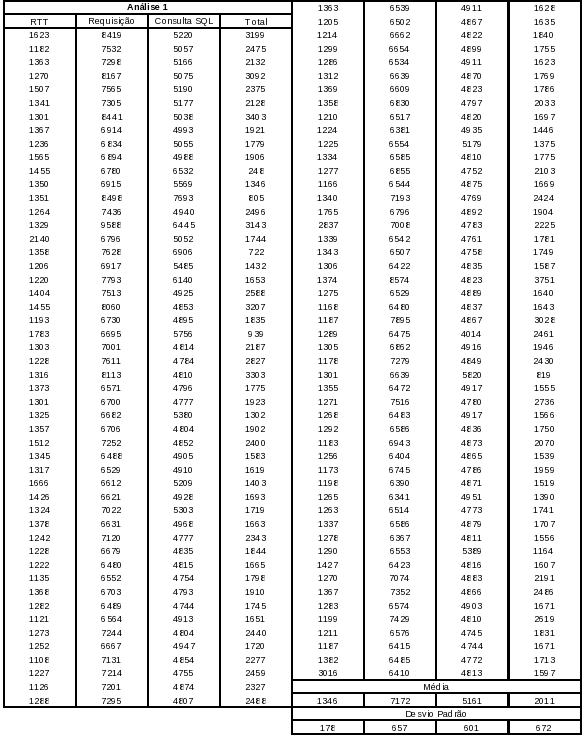
\includegraphics[width=15cm]{analise1.png} 
  \caption{Representação das medições da análise 1.}
  \label{fig:analise1}
\end{figure}

\textbf{Análise 2: }\\
Média do tempo de RTT: \textbf{1293 us}\\
Desvio padrão RTT: \textbf{335 us}\\
Média do tempo total de requisição: \textbf{1932 us}\\
Desvio padrão de requisição: \textbf{909 us}\\
\begin{figure}[htb]
  \centering
  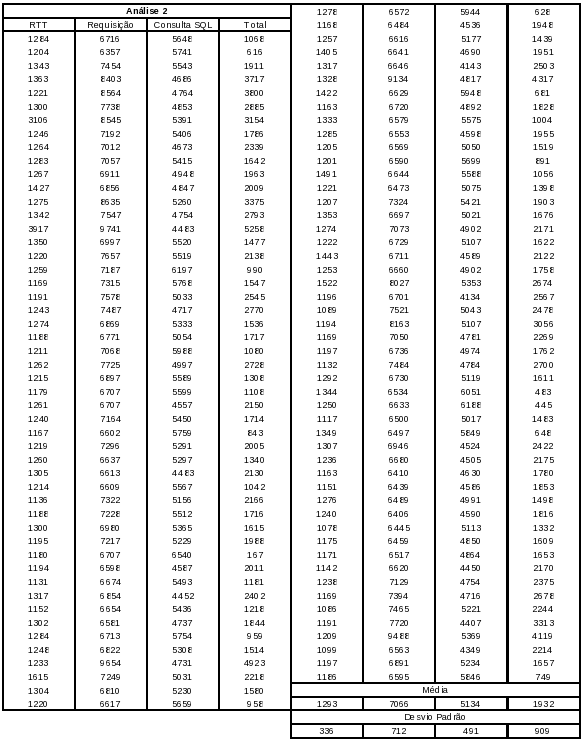
\includegraphics[width=15cm]{analise2.png} 
  \caption{Representação das medições da análise 2.}
  \label{fig:analise2}
\end{figure}

\textbf{Análise 3: }\\
Média do tempo de RTT: \textbf{1355 us}\\
Desvio padrão RTT: \textbf{182 us}\\
Média do tempo total de requisição: \textbf{2043 us}\\
Desvio padrão de requisição: \textbf{864 us}\\
\begin{figure}[htb]
  \centering
  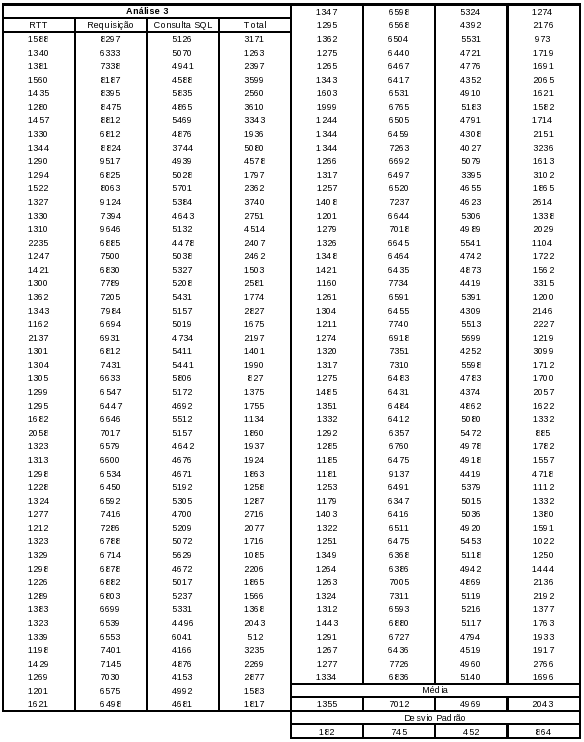
\includegraphics[width=15cm]{analise3.png} 
  \caption{Representação das medições da análise 3.}
  \label{fig:analise3}
\end{figure}

\textbf{Análise 4: }\\
Média do tempo de RTT: \textbf{1424 us}\\
Desvio padrão RTT: \textbf{606 us}\\
Média do tempo total de requisição: \textbf{2065 us}\\
Desvio padrão de requisição: \textbf{868 us}\\
\begin{figure}[htb]
  \centering
  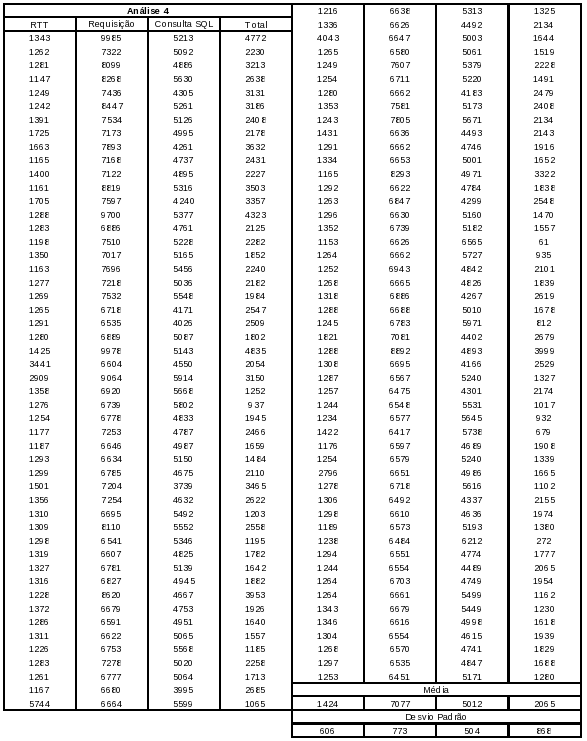
\includegraphics[width=15cm]{analise4.png} 
  \caption{Representação das medições da análise 4.}
  \label{fig:analise4}
\end{figure}

\textbf{Análise 5: }\\
Média do tempo de RTT: \textbf{1338 us}\\
Desvio padrão RTT: \textbf{369 us}\\
Média do tempo total de requisição: \textbf{1974 us}\\
Desvio padrão de requisição: \textbf{846 us}\\
\begin{figure}[htb]
  \centering
  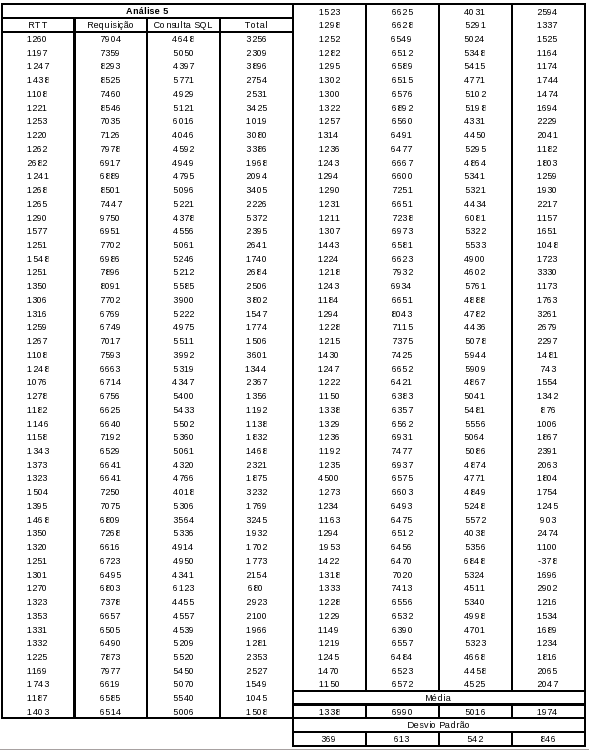
\includegraphics[width=15cm]{analise5.png} 
  \caption{Representação das medições da análise 5.}
  \label{fig:analise5}
\end{figure}

\subsection{Comparação dos projetos feitos em Java RMI e em Sockets TCP em C }

As diferenças mais relevantes entre os dois projetos são:\\
- \textbf{Nível de Abtração}: Em Java o nível de abstração é alto, e foi fácil implementar o sistema já que toda parte de comunicação TCP já vem pronta e não necessita um controle mais intensivo, utilizando aproximadamente 500 linhas de código, porém, roda sobre uma máquina virtual que costuma ser responsável por quedas no desempenho. Já em C, o nível de abstração é baixo, pois é necessário configurar todos os detalhes da comunicação TCP e é muito suscetível a erros, sendo mais trabalhoso de se implementar, também utilizou aproximadamente 1500 linhas de código, 3 vezes mais linhas que o sistema feito em Java, porém, o ganho deste trabalho é um maior poder de controle e maior velocidade.\\
- \textbf{Implementação do Banco de Dados}: Em C, utilizamos um arquivo simples para armazenar nossos dados, e em Java utilizamos um programa de banco de dados sql.\\
Para fazer a análise de tempo, primeiro temos que relembrar os tempos obtidos no mesmo projeto mas feito com Sockets TCP em C, que foram:

Média do tempo de RTT: \textbf{274,16 us}\\
Desvio padrão: \textbf{10,72 us}\\
Média do tempo de consulta: \textbf{1769,16 us}\\
Desvio padrão: \textbf{432,29 us}\\

Podemos notar que o tempo de RTT em C é muito menor do que em Java, como já era de se esperar já que em C não é necessário se rodar o sistema em uma máquina virtual além de uma implementação que é mais eficiênte por ser de mais baixo nível. Já no tempo de consulta, temos resultados interessantes, pois em Java foi muito próximo dos tempo obtidos em C, que vai contra o esperado, mas isso pode ser explicado por causa da implementação do banco de dados. Um sistema de banco de dados sql é uma forma otimizada de se armazenar dados, o que é muito mais eficiênte que se abrir, fechar e manipular arquivos em disco, e por isso os resultados de tempo obtidos em Java foram próximos dos tempos em C.\\
Analisando o desempenho geral dos dois sistemas, os prós e contras de cada um fizeram com que ambos tivessem um desempenho bem similar, e que assim, a escolha de qual sistema utilizar vem da escolha de cada usuário.\\ 

\section{Confiabilidade e Consistência}
Dois pontos a considerar: robustez quanto à comunicação e consistência dos dados.\\
Tentamos fazer todas as verificações de erros possíveis nas funções das bibliotecas de comunicação com o socket, tanto no lado cliente como no servidor. Ainda assim, não conseguimos implementar um importante caso de exceção: notificar e encerrar o cliente quando o servidor "cai".\\
Com relação à consistência dos dados, esta é garantida pela exclusão mútua nas operações de atualização de avaliação.\\

\section{Conclusão}
Podemos considerar que a aplicação já está totalmente funcional, todas as consultas estão funcionando corretamente, há a garantia da consistência do banco de dados do cinema e a comunicação entre cliente e servidor está boa, tendo também a garantia que se o servidor cai, o cliente é notificado do erro.\\
Além de não ter sido transparente o jeito que é implementado a comunicação, ela é feita interiormente por protocolo TCP, e por utilizar o protocolo TCP, a comunicação possui todas as suas vantagens, como confiabilidade na transferência de pacotes, controle de fluxo e controle de congestionamento, o que garante uma qualidade maior à aplicação.\\
A análise de tempo foi bem interessante, já que por utilizar um banco de dados sql ao invés de manipular arquivos, teve um desempenho similar ao projeto feito em C.\\
Ao fazer a aplicação em Java, o nível de abstração foi alto, pois não tivemos que tratar muitos detalhes das conexões.\\
Outra vantagem trazida pelo alto nível de abstração é a exclusão mútua já ser implementada no banco de dados sql, facilitando mais a implementação do sistema.\\
Nosso servidor de banco de dados de cinema ainda não é um sistema completo e bem acabado, mas já provê uma base sólida para implementar aplicações gráficas e de maior porte, utilizando o servidor como o núcleo da aplicação. Pretendemos, em versões posteriores, melhorar o programa, resolver bugs e talvez, utilizar uma biblioteca gráfica para tornar sua interface mais usável.\\

\section{Código Fonte}

%%%%%%%%%%%%%%%%%%%%%%%%%%%%%%%%%%%%%%%%%%
%%%%%%% runserver.sh
\subsection{runserver.sh}  % 1
\begin{verbatim}
#!/bin/bash

ROOTDIR=$(pwd) #/home/ec2007/..../mc823-1s2010/proj3
CLASSPATH=$CLASSPATH:$ROOTDIR/sqlitejdbc-v056.jar

cd bin

# executa o servidor passando como parâmetro o arquivo do BD
java -Djava.security.policy=$ROOTDIR/policy Servidor $ROOTDIR/filmes.db
\end{verbatim}


%%%%%%%%%%%%%%%%%%%%%%%%%%%%%%%%%%%%%%%%%%
%%%%%%% runclient.sh
\subsection{runclient.sh} % 2
\begin{verbatim}
#!/bin/bash

cd bin

# $# - número de parametros 
if [ $# -ne 1 ]
then
    echo "uso: ./runclient.sh <endereço_servidor>"
    exit 1
fi

# $1 - endereço do servidor
java -Djava.security.policy=../policy Cliente $1
\end{verbatim}


%%%%%%%%%%%%%%%%%%%%%%%%%%%%%%%%%%%%%%%%%%
%%%%%%% teste_server.sh
\subsection{teste_server.sh} % 3
\begin{verbatim}
#!/bin/bash

OUT=tempos.server

# limpa o arquivo com os tempos antigos
rm $OUT

./runserver.sh 2>> $OUT
\end{verbatim}


%%%%%%%%%%%%%%%%%%%%%%%%%%%%%%%%%%%%%%%%%%
%%%%%%% teste_conexao.sh
\subsection{teste_conexao.sh}     % 4
\begin{verbatim}
#!/bin/bash

# $# - número de parametros 
if [ $# -ne 1 ]
then
    echo "uso: ./teste_conexao.sh <endereço_servidor>"
    exit 1
fi

OUT=tempos.rtt

# limpa o arquivo com os tempos antigos
rm $OUT

for i in $(seq 500)
do
  ./runclient.sh $1 <file.in 2>> $OUT
done

clear
echo "$OUT gerado"
echo "Lembrete da condição:"
echo "(Client.java) boolean TEST = false;"
\end{verbatim}


%%%%%%%%%%%%%%%%%%%%%%%%%%%%%%%%%%%%%%%%%%
%%%%%%% teste_consulta.sh
\subsection{teste_consulta.sh}      % 5 
\begin{verbatim}
#!/bin/bash

# $# - número de parametros 
if [ $# -ne 1 ]
then
    echo "uso: ./teste_consulta.sh <endereço_servidor>"
    exit 1
fi

OUT=tempos.query

# limpa o arquivo com os tempos antigos
rm $OUT

./runclient.sh $1 2>> $OUT

clear

# lembrete pra quando for rodar o teste
echo "$OUT gerado"
echo "Lembrete da condição:"
echo "(Client.java) boolean TEST = true;"

\end{verbatim}


%%%%%%%%%%%%%%%%%%%%%%%%%%%%%%%%%%%%%%%%%%
%%%%%%% policy
\subsection{policy}       % 6
\begin{verbatim}
grant {
      // totalmente permissivo - apenas exemplo
      permission java.security.AllPermission;
};
\end{verbatim}


%%%%%%%%%%%%%%%%%%%%%%%%%%%%%%%%%%%%%%%%%%
%%%%%%% cliente.java
\subsection{Cliente.java}       % 7
\begin{verbatim}
import java.io.IOException;
import java.rmi.RemoteException;
import java.rmi.registry.LocateRegistry;
import java.rmi.registry.Registry;
import java.sql.SQLException;


public class Cliente {

	// número da porta que o servidor usará
	private static final int serverPort = 3232;
	
	// constantes para a seção de teste
	private static final boolean TEST = false;
	private static final int DEFAULT_OPT = ClientAux.LISTAR_TODOS_COMPLETO;
	private static final int TEST_ITERATIONS = 500;
	
	
    static public void main(String args[]) throws IOException, SQLException {

    	// o cliente tem acesso à interface para o objeto remoto
		RequestInterface servidor = null;
    	Registry registry;
    	
    	// endereço é passado como argumento
    	String serverAddress = args[0];

    	// estabelece comunicação com o objeto remoto
    	try {
        	// recebe o "registry" pelo endereço e porta
        	registry = LocateRegistry.getRegistry(serverAddress, serverPort);
        	// busca pelo objeto remoto
        	servidor = (RequestInterface) registry.lookup("servidor");
    	} 

    	// tratamento das possíveis exceções
    	catch(RemoteException e) {
    		System.err.println("Não foi possível localizar o objeto remoto.");
    		//e.printStackTrace();
    		System.out.println("Servidor não disponível.");
    		System.exit(1);
    	} catch(Exception e) {
    		e.printStackTrace();
    		System.exit(1);
    	}
    	
    	
    	// a partir daqui, se o cliente conseguiu encontrar o objeto remoto,
    	// então pode-se realizar as chamadas para os métodos remotos
    	long t1,t2;
    	
    	// faz a contagem do tempo de RTT
    	t1 = System.nanoTime();
    	// notifica o servidor da conexão
    	servidor.sayHello();  
		t2 = System.nanoTime();
		System.err.println( ( (t2-t1)/1000 ) );
    	
    	int option;
    	
    	// loop principal do cliente
		if(!TEST) {
	    	option = ClientAux.readOption();
		}
    	// [início] Seção de teste
    	// tivemos dificuldade em gerar um script para a automação do teste 
    	// de sucessivas consultas. Desconsiderar esta seção
		else {
    		option = DEFAULT_OPT;
    		for(int i = 0; i < TEST_ITERATIONS; i++) {
        		ClientAux.makeRequest(servidor, option);
    		}
    		option = ClientAux.SAIR;
    	}
    	// [fim] Seção de teste
    	
    	while(option != ClientAux.SAIR) {
    		try {
        		ClientAux.makeRequest(servidor, option);
    		} catch(RemoteException e) {
        		System.out.println("Servidor não disponível.");
        		System.exit(1);
    		} catch(Exception e) {
    			System.out.println("Algum erro ocorreu no servidor.");
        		System.exit(1);
    		}
    		
    		option = ClientAux.readOption();
    	}

    	return; // main cliente

    }

    	
}
\end{verbatim}


%%%%%%%%%%%%%%%%%%%%%%%%%%%%%%%%%%%%%%%%%%
%%%%%%% ClientAux.java
\subsection{ClientAux.java}       % 8
\begin{verbatim}
import java.io.BufferedReader;
import java.io.IOException;
import java.io.InputStreamReader;
import java.rmi.RemoteException;
import java.sql.SQLException;
import java.util.List;

import bd.Filme;


public class ClientAux {

	// --- Constantes ---
	static final int LISTAR_TODOS_COMPLETO = 1;
	static final int LISTAR_TODOS = 2;
	static final int REG_COMPLETO = 3;
	static final int REG_SINOPSE = 4;
	static final int REG_MEDIA = 5;
	static final int REG_AVALIAR = 6;
	static final int SAIR = 7;
	// --- Constantes ---
	
	
	// método auxiliar para interface e leitura da opção
	public static int readOption() throws IOException {
		
		// objeto para leitura
		BufferedReader in = new BufferedReader(new InputStreamReader(System.in));

		System.out.println("\n====================================================\n");
		System.out.println("Escolha uma entre as opções e tecle Enter:");
		System.out.println(" [1] Listar todas as informações de todos os filmes.");
		System.out.println(" [2] Listar id e título de todos os filmes.");
		System.out.println(" [3] Listar todas as informações de um filme.");
		System.out.println(" [4] Mostrar a sinopse de um filme.");
		System.out.println(" [5] Mostrar a avaliação de um filme.");
		System.out.println(" [6] Avaliar um filme!");
		System.out.println(" [7] Sair");
		
		// tenta fazer o parse da string digitada para inteiro. Se funcio-
		// nar, retorna o valor; caso contrário, chama novamente a função
		try {
			return Integer.parseInt(in.readLine());
		} catch (NumberFormatException e) {
			return readOption();
		}

	}

	// método para interface com o usuário e leitura de Id
	private static int readId() throws IOException {
		System.out.print("  Id: ");
		BufferedReader in = new BufferedReader(new InputStreamReader(System.in));
		try {
			return Integer.parseInt(in.readLine());
		} catch (NumberFormatException e) {
			return readOption();
		}
	}
	
	private static float readNota() throws IOException {
		System.out.print("  Nota: ");
		BufferedReader in = new BufferedReader(new InputStreamReader(System.in));
		try {
			return Float.parseFloat(in.readLine());
		} catch (NumberFormatException e) {
			return readNota();
		}
	}
	
	// método que seleciona a opção e realiza as chamadas ao servidor
	public static void makeRequest(RequestInterface servidor, int option) 
		throws SQLException, IOException, RemoteException {
		
		// variável para retorno das consultas
		List<Filme> listaFilmes;
		
		int idProcurado;
		float novaNota;
		long t1,t2;
		
		// seleciona o que será executado a partir da opção de entrada
		switch (option) {
		case LISTAR_TODOS_COMPLETO:
			// inicia a contagem de tempo de requisição
			t1 = System.nanoTime();
			
			// faz a requisição de todos os filmes ao servidor
			listaFilmes = servidor.getFullList();
			
			// termina a contagem do tempo
			t2 = System.nanoTime();
			System.err.println( ( (t2-t1)/1000 ) );
			
			// para cada filme na lista retornada, imprime as informações
			for(Filme f : listaFilmes) {
				f.printFullInfo();
			}
			break;
		case LISTAR_TODOS:
			// cliente requisita todos os campos de todos os filmes
			// ao servidor, mas imprime apenas os campos ID e Nome
			listaFilmes = servidor.getFullList();
			
			for(Filme f : listaFilmes) {
				f.printIdNome();
			}
			break;
		case REG_COMPLETO:
			idProcurado = readId();
			// faz a requisição por um filme específico
			listaFilmes = servidor.getFilmeById(idProcurado);
			// o retorno da busca por um filme é uma lista, de modo
			// que é possível verificar se a mesma está vazia ou não
			if(listaFilmes.isEmpty()) System.out.println("  Filme não encontrado!");
			else listaFilmes.get(0).printFullInfo();
			break;
		case REG_SINOPSE:
			idProcurado = readId();
			listaFilmes = servidor.getFilmeById(idProcurado);
			if(listaFilmes.isEmpty()) System.out.println("  Filme não encontrado!");
			else listaFilmes.get(0).printSinopse();
			break;
		case REG_MEDIA:
			idProcurado = readId();
			listaFilmes = servidor.getFilmeById(idProcurado);
			if(listaFilmes.isEmpty()) System.out.println("  Filme não encontrado!");
			else listaFilmes.get(0).printNota();
			break;
		case REG_AVALIAR:
			idProcurado = readId(); // leitura do id do filme a avaliar
			novaNota = readNota(); // nota a ser dada para o filme
			if(servidor.avaliaFilme(idProcurado, novaNota)) {
				System.out.println("  Avaliação realizada com sucesso!");
			} else {
				System.out.println("  Filme não encontrado!");
			}
			break;
		}
		
	}
}
\end{verbatim}



%%%%%%%%%%%%%%%%%%%%%%%%%%%%%%%%%%%%%%%%%%
%%%%%%% RequestInterface.java
\subsection{RequestInterface.java}       % 9
\begin{verbatim}
import java.rmi.Remote;
import java.rmi.RemoteException;
import java.sql.SQLException;
import java.util.List;

import bd.Filme;

// esta é a interface que define os métodos remotos 
// implementados pelo servidor 
public interface RequestInterface extends Remote {
	
	// Notificar que alguem se conectou no servidor
	// Método "leve", isto é, sem parâmetros nem retorno. É usado para encontrar 
	// o tempo de comunicação base do RMI, isto é, o tempo para chamada de método
	void sayHello() throws RemoteException;
	
	//Retornar a lista completa de todos os filmes
	List<Filme> getFullList() throws RemoteException, SQLException;
	
	//Retornar uma lista, que pode ser vazia se não encontrou o elemento, ou ter 
	// 1 elemento caso contrario
	List<Filme> getFilmeById(Integer idProcurado) throws 
		RemoteException, SQLException;
	
	//Receber uma avaliação e atualizar a nota do filme
	Boolean avaliaFilme(Integer idFilme, Float novaNota) throws 
		RemoteException, SQLException;
	
}
\end{verbatim}



%%%%%%%%%%%%%%%%%%%%%%%%%%%%%%%%%%%%%%%%%%
%%%%%%% Servidor.java
\subsection{Servidor.java}       % 10
\begin{verbatim}
import java.rmi.RemoteException;
import java.rmi.registry.LocateRegistry;
import java.rmi.registry.Registry;
import java.rmi.server.UnicastRemoteObject;
import java.sql.SQLException;
import java.util.List;

import bd.ConnectionFactory;
import bd.DataAccess;
import bd.Filme;


@SuppressWarnings("serial")
public class Servidor extends UnicastRemoteObject 
	implements RequestInterface {

	private static int port = 3232;
	private Registry registry;

	// ========== Construtor ==========
	public Servidor() throws RemoteException {

		// cria o registry na porta especificada
		registry = LocateRegistry.createRegistry(port);
		// faz o bind para o nome do objeto
		registry.rebind("servidor", this);
		
		System.out.println("Aguardando requisições...");
		
		return;
	}
	
	// ========== Main ==========
	public static void main(String[] args) throws SQLException {

		// o servidor é executado com o caminho do arquivo do
		// BD como primeiro e único parâmetro
		ConnectionFactory.caminhoAbsolutoBd = args[0];

		try {
			@SuppressWarnings("unused")
			Servidor s = new Servidor();
		} catch (Exception e) {
			e.printStackTrace();
			System.exit(1);
		}
	
		return;
	}
	
	
	// ========== Métodos remotos que o servidor implementa ==========
	public void sayHello() {
		System.out.println("Algum cliente se conectou.");
	}

	public List<Filme> getFullList() throws RemoteException, SQLException {
		return DataAccess.getFullList();
	}
	
	public List<Filme> getFilmeById(Integer idProcurado) throws SQLException {
		return DataAccess.getFilmeById(idProcurado);
	}

	public Boolean avaliaFilme(Integer idProcurado, Float novaNota) throws SQLException {
		return DataAccess.avaliaFilme(idProcurado, novaNota);
	}

}
\end{verbatim}


%%%%%%%%%%%%%%%%%%%%%%%%%%%%%%%%%%%%%%%%%%
%%%%%%% ConnectionFactory.java
\subsection{ConnectionFactory.java}       % 11
\begin{verbatim}
package bd;

import java.sql.Connection;
import java.sql.DriverManager;
import java.sql.SQLException;

public class ConnectionFactory {
	
	public static String caminhoAbsolutoBd;
	
	public static Connection getConnection() throws SQLException {

		Connection con = null;

		try {
			Class.forName("org.sqlite.JDBC");
			con =  DriverManager.getConnection("jdbc:sqlite:" + caminhoAbsolutoBd);
		} catch (ClassNotFoundException e) {
			e.printStackTrace();
		}

		return con;
		
	}

}
\end{verbatim}


%%%%%%%%%%%%%%%%%%%%%%%%%%%%%%%%%%%%%%%%%%
%%%%%%% DataAccess.java
\subsection{DataAccess.java}       % 12
\begin{verbatim}
package bd;

import java.sql.Connection;
import java.sql.PreparedStatement;
import java.sql.ResultSet;
import java.sql.SQLException;
import java.util.ArrayList;
import java.util.List;

// esta classe é responsável por fazer a interface com o banco de dados
// aqui se encontram os comandos SQL responsáveis pelas consultas ao e 
// alterações no banco
public class DataAccess {

	// Métodos usados pelo Servidor para acesso aos dados	
	
	// retorna a lista de todos os filmes no banco
	public static List<Filme> getFullList() throws SQLException {
		
		long t1,t2;
		
		// inicia a contagem do tempo de consulta
    	t1 = System.nanoTime();
    	
		// abre a conexão com o banco
		Connection con = ConnectionFactory.getConnection();

		// preparo do comando sql de consulta
		String sql = "SELECT * FROM filme;";
		PreparedStatement stmt = con.prepareStatement(sql);
		ResultSet rs = stmt.executeQuery();

		List<Filme> listaFilmes = new ArrayList<Filme>();

		// popula a lista com o resultado da consulta
		while(rs.next()) {
			// instancia e popula o objeto filme
			Filme f = new Filme();
			f.buildBeanByRs(rs);
			// e o adiciona na lista
			listaFilmes.add(f);
		}

		stmt.close();
		con.close(); // fecha a conexão
		
		//termina a contagem do tempo de consulta
		t2 = System.nanoTime();
		System.err.println( ( (t2-t1)/1000 ) );
		
		return listaFilmes;
	}

	// consulta a filme a partir do seu ID:
	// retorna uma lista ou vazia ou com um único elemento
	public static List<Filme> getFilmeById(Integer idProcurado) throws SQLException {

		// abre a conexão com o banco
		Connection con = ConnectionFactory.getConnection();
		
		// preparo do comando sql de consulta
		String sql = "SELECT * FROM filme WHERE id=?;";
		PreparedStatement stmt = con.prepareStatement(sql);
		stmt.setInt(1, idProcurado);
		ResultSet rs = stmt.executeQuery();

		List<Filme> listaFilmes = new ArrayList<Filme>();

		// se houver algum filme com o id procurado, insere-o na lista
		if(rs.next()) {
			Filme f = new Filme();
			f.buildBeanByRs(rs);
			listaFilmes.add(f);
		}

		stmt.close();
		con.close(); // fecha a conexão com o banco
		return listaFilmes;
	}


	// realiza a atualização da nota, retornando true se a operação for
	// bem-sucedida (ie, se o filme solicitado existe)
	public static boolean avaliaFilme(Integer idProcurado, Float novaNota)
		throws SQLException {

		// abre a conexão com o banco
		Connection con = ConnectionFactory.getConnection();
		
		// preparo do comando sql de consulta
		String sql = "SELECT * FROM filme WHERE id=?;";
		PreparedStatement stmt = con.prepareStatement(sql);
		stmt.setInt(1, idProcurado);
		ResultSet rs = stmt.executeQuery();
		
		// se não houver nenhum elemento na consulta, termina
		if(!rs.next()) {
			stmt.close();
			con.close();
			return false;
		}

		// lê a nota e o n de aval atuais
		float nota = rs.getFloat("nota");
		int n_avaliacoes = rs.getInt("n_avaliacoes");
		
		// faz a média ponderada das notas que já foram dadas
		nota = ((nota * n_avaliacoes) + novaNota) / (n_avaliacoes + 1);
		n_avaliacoes++;
		
		// preparo do comando sql de atualização
		sql = "UPDATE filme SET nota=?, n_avaliacoes=? WHERE id=?";
		stmt = con.prepareStatement(sql);
		stmt.setFloat(1, nota);
		stmt.setInt(2, n_avaliacoes);
		stmt.setInt(3, idProcurado);
		stmt.execute(); // executa a operação
		
		stmt.close();
		con.close(); // fecha a conexão com o banco

		return true;
	}

}
\end{verbatim}


%%%%%%%%%%%%%%%%%%%%%%%%%%%%%%%%%%%%%%%%%%
%%%%%%% Filme.java
\subsection{Filme.java}       % 13
\begin{verbatim}
package bd;

import java.io.Serializable;
import java.sql.ResultSet;
import java.sql.SQLException;

@SuppressWarnings("serial")
public class Filme implements Serializable {

	// atributos do filme
	private int id;
	private int n_avaliacoes;
	private float nota;
	private String titulo;
	private String sinopse;
	private String salas;
	
	// método público para recuperar id de um filme
	public int getId() {
		return id;
	}
	

	// método de população do objeto que representa um registro (bean)
	// a partir do ResultSet retornado da consulta SQL
	public void buildBeanByRs(ResultSet rs) throws SQLException {
		this.id = rs.getInt("id");
		this.n_avaliacoes = rs.getInt("n_avaliacoes");
		this.nota = rs.getFloat("nota");
		this.titulo = rs.getString("titulo");
		this.sinopse = rs.getString("sinopse");
		this.salas = rs.getString("salas");
		return;
	}
	
	// métodos de impressão das informações de um filme
	public void printFullInfo() {
		System.out.println("  Id: " + getId() + " | Título: " + titulo);
		System.out.println("  Sinopse: " + sinopse);
		System.out.println("  Salas: " + salas);
		if (n_avaliacoes != 0) {
			// aval recebe 'avaliação' (exatamente UMA) ou 'avaliações' (>1)
			String aval = (n_avaliacoes > 1) ? "avaliações" : "avaliação";
			System.out.println("  Nota: " + nota + " (a partir de " + 
					n_avaliacoes + " " + aval + ")");
		} else {
			System.out.println("  Ainda não há avaliações para este filme.");
		}
		System.out.println("___");
		return;
	}
	public void printIdNome() {
		System.out.println("  Id: " + getId() + " | Título: " + titulo + "\n___");
		return;
	}
	public void printSinopse() {
		System.out.println("  Sinopse: " + sinopse);
	}
	public void printNota() {
		if (n_avaliacoes != 0) {
			String aval = (n_avaliacoes > 1) ? "avaliações" : "avaliação";
			System.out.println("  Nota: " + nota + " (a partir de " + 
					n_avaliacoes + " " + aval + ")");
		} else {
			System.out.println("  Ainda não há avaliações para este filme.");
		}
		return;
	}


}
\end{verbatim}


\section{Anexo}
%\begin{figure}[htb]
%  \centering
%  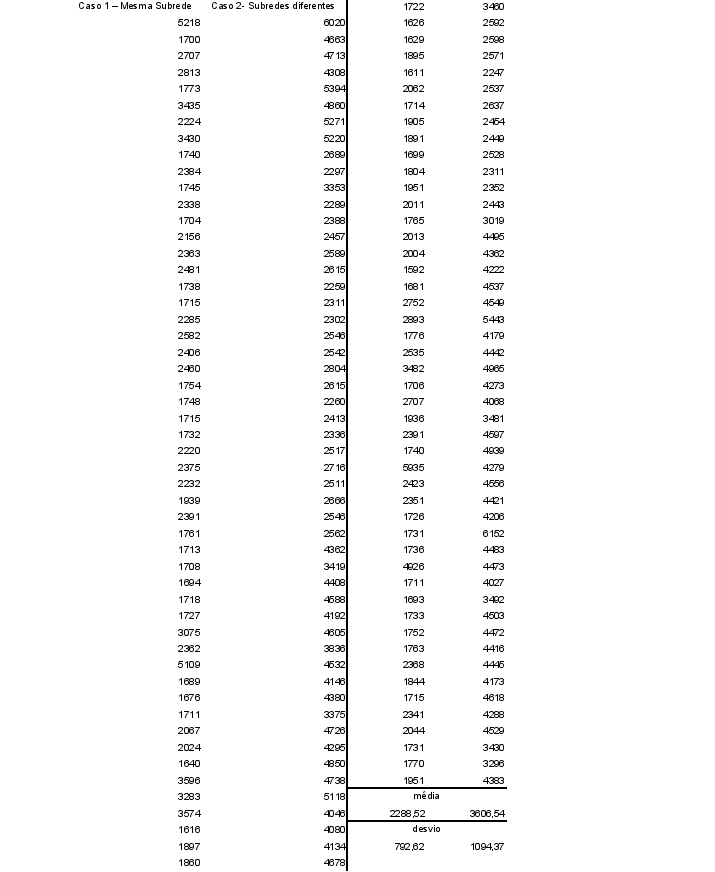
\includegraphics[width=15cm]{medicoes.png} 
%  \caption{Representação das medições para a consulta.}
%  \label{fig:rtt}
%\end{figure}

\begin{thebibliography}{99}
\bibitem{R1} HALL, Brian. Beej's Guide to Network Programming. Disponível em: http://http://beej.us/guide/bgnet/output/html/multipage/index.html.
\end{thebibliography}

\end{document}
